\chapter{はじめに}
\label{ch:intro}

\quad

\section{研究背景}
\label{sec:research_bg}

日本企業の RPA (Robotics Process Automation~\cite{yasuhiro2017rpa})導入率は全体で38\%,中小企業では25\%となっており,非常に少ないことがわかる(図~\ref{fig:rpa_rate}).
また,大企業と中小企業の間に20\%以上の差があり,技術や規模による格差も見て取れる.
これらの原因となっており要因として考えられることは,大きく分けて2つある.1つ目は,RPAには専門領域と非専門領域が存在するということである.
専門領域はPC上の操作や,デジタルの領域における処理である.いっぽうで,紙媒体の処理等の,アナログの世界で行われる処理は非専門領域としている.
特に,手書きの文字や画像の認識を高い精度を保ちながら自動で行うことは,現代では非常に困難なことである.具体的には,縦書き文字横書き文字が混在していたり,旧字体や特殊文字等の組み合わせも考えられるため,例外的な処理までを自動で行う必要があるからである~\cite{d-analyzer2019rpa}.
2つ目の原因は,紙媒体の業務を行っているコミュニティのIT知識の乏しさにある.詳しくは次のセクションで説明する.このような現状を踏まえて,次章からは,OCR技術を使用したアプローチを提案する.
また, RPA の定義についても,明確には定まっていない部分が多い.自動化という概念自体に対して RPA という言葉を適用するとしたら,工場で食品の生産や梱包を行うロボットも,我々の家で活躍するお掃除ロボットも, PC 上のボタン一つで複数の処理を行うシステムも全て RPA と呼ぶことができる.
そのため,本研究では, RPA という言葉の意味を広義的に捉え, RPA の非専門領域で行われる処理を,他の様々な技術を用いて克服することを目標とする.
より詳細な技術については第\ref{ch:rw}章で述べるが, OCR や 字句解析の技術を使用し,紙媒体に対する処理を不自由なく自動化し, Ruby on Rails を使用したシステムとしての運用を行い,我々の周りに多くある Web アプリケーションと同様に利用できるようにすることで,
IT に関する知識が乏しいコミュニティでも,安全かつ快適に自動化の恩恵を受けることを目指す.

\clearpage
\begin{figure}[htbp]
\centering
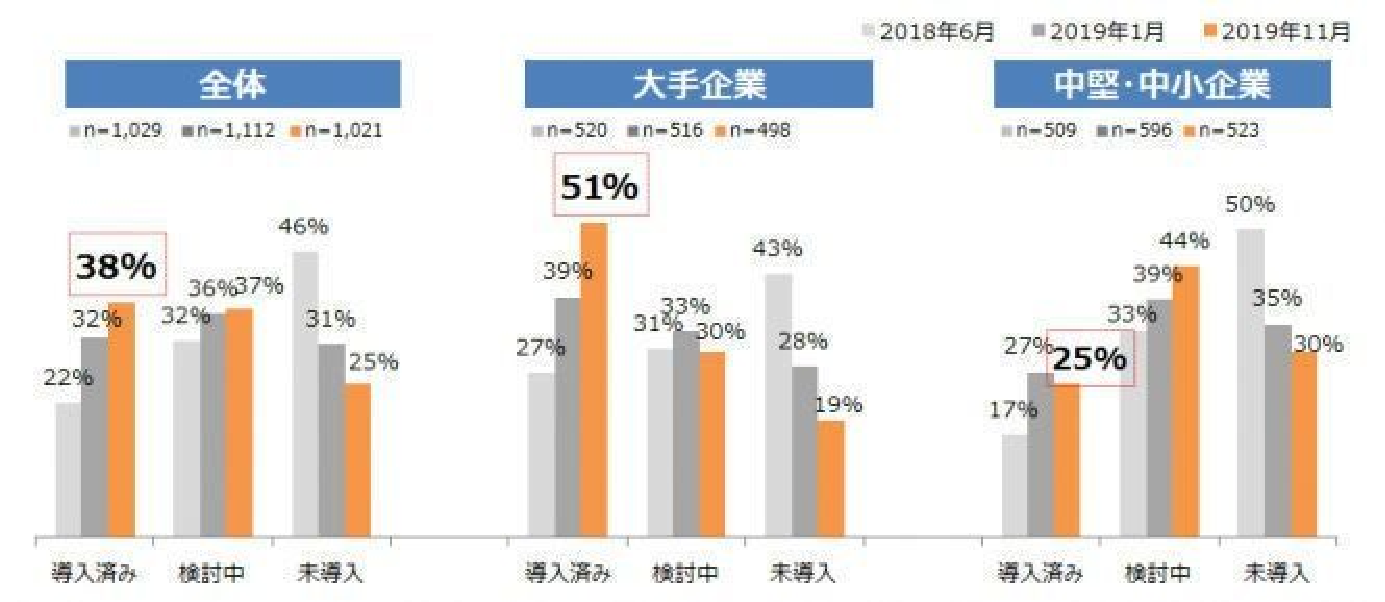
\includegraphics[scale = 0.6]{img/rpa_rate.pdf}
\caption{企業のRPA導入率}
\label{fig:rpa_rate}
\end{figure}%

\section{研究目的}
\label{sec:research_purpose}

本研究の目的は,IT知識が乏しく,紙媒体の業務を行っているコミュニティを中心に, RPA を使用して紙媒体の処理を自動で行うシステムを作成することである.
具体的な内容に入る前に,紙媒体の業務とIT知識の関連性について深堀りする.
日本で働く人事 ・ 総務担当者に,「紙媒体中心の業務で不便を感じたことがあるか?」とアンケートを取ったところ,61\%が不便を感じたことがあると回答した(図~\ref{fig:paper_media_survey}).上記の理由として,システム障害への恐怖感や,IT知識の乏しさが挙げられます.しかし,一連の流れをRPAにすることで,IT知識の有無に関わらず,システムを運用することを目指す.


\begin{figure}[htbp]
  \vspace{1cm}
  \centering
  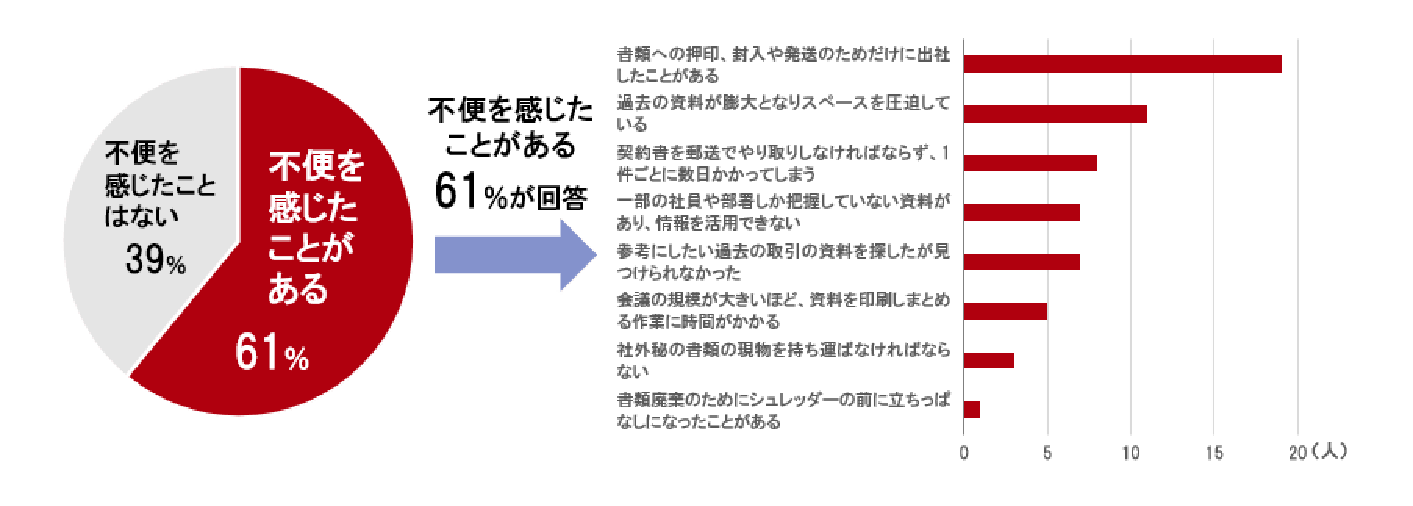
\includegraphics[scale = 0.6]{img/paper_media_survey.pdf}
  \caption{紙媒体中心業務に関するアンケート}
  \label{fig:paper_media_survey}
\end{figure}%

\section{構成}
\label{sec_str}

本論文は6章構成になっている.第\ref{ch:intro}章では,本研究の背景や目的を述べる.
第\ref{ch:rw}章では既存手法との比較や課題を述べる.
本研究での実装手法を第\ref{ch:app}章で提案し,第\ref{ch:exp}章で実験と評価,第\ref{ch:eval}章で結果の考察を述べ,第\ref{ch:con}章でに本研究の総括を行う.
